\documentclass{article}
\usepackage[utf8]{inputenc} % para que nos acepte la codificación UTF-8
\usepackage[spanish]{babel} % establecemos el idioma del documento al español
\usepackage{graphicx,float}

\begin{document}
\title{Practica 5. Modelos de la Computación}
\author{Pablo Navarro}
\maketitle
\section{Practica 5}
\subsection{Ejercicio 1}
Dada la gramática: \\
$S\ \rightarrow\ a \mid\ S1 \mid \qquad \qquad \qquad \qquad S\ \rightarrow a\ S4\ d\ S5 \\
S1\ \rightarrow a\ \mid\ S1\ \mid\ d\ \mid\ b\ S2\ \qquad \ S4\ \rightarrow\ a\ S4\ \mid\ b\ S6\ c \\
S2\ \rightarrow\ b S2 \mid c \ S3 \qquad \qquad \qquad \quad S5 \rightarrow \ d \mid S5 \mid d \\
S3\ \rightarrow\ c\ S3\ \mid\ \varepsilon \qquad \qquad \qquad \qquad \ \ S6\rightarrow\ b\ S6\ c\ \mid \varepsilon $

\begin{itemize}
  \item [A] Demuestra que la gramática es ambigua:\\
        Es ambigua porque hay palabras que tienen dos árboles de derivación distintos

        \begin{figure}[H]
          \centering
          \includegraphics[width=0.8\textwidth]{fotos/derivacion1}
        \end{figure}

        $S \longrightarrow aabcdd$
  \item [B] Determina el lenguaje que genera la gramática\\
        $L=\{a^nb^nc^od^n\ :\ n >= 1,\ m >= 1,\ o >= 1\ \cup
        \ a^nb^mc^md^o\ :\ n >= 1,\ m >= 1,\ o >= 2\}$
  \item [C] Encuentra una gramática no ambigua que genere el mismo lenguaje\\
        $S\ \rightarrow\ a\ S2\\
        S2\ \rightarrow\ b\ S3\\
        S3\ \rightarrow\ c\ S4\\
        S4\ \rightarrow\ d\\
        \\
        S5\ \rightarrow\ a\ S6\ d\\
        S6\ \rightarrow\ a\ S7\ d\ \mid\ b\ S8\ c\\
        S7\ \rightarrow\ a\ S7\ d\ \mid\ b\ S9\ c\\
        S8\ \rightarrow\ b\ S9\ c\\
        S9\ \rightarrow\ b\ S9\ c\ \mid\ \varepsilon\\
        \\
        S10\ \rightarrow\ a\ S11\ d\\
        S11\ \rightarrow\ a\ S11\ d\ \mid\ b\ S12\ c\\
        S12\ \rightarrow\ b\ S12\ c\ \mid\ b\ S13\ \mid\ S14\ c\\
        S13\ \rightarrow\ b\ S13\ \mid\ \varepsilon\\
        S14\ \rightarrow\ S14\ c\ \mid\ \varepsilon\\
        \\
        S15\ \rightarrow\ S16\ d\\
        S16\ \rightarrow\ a\ S16\ d\ \mid\ a\ S17\ d\\
        S17\ \rightarrow\ b\ S18\ c\ \mid\ a\ S19\\
        S18\ \rightarrow\ b\ S18\ c\ \mid\ \varepsilon\\
        S19\ \rightarrow\ a\ S20 \\
        S20\ \rightarrow\ a\ S20\ \mid\ S18\\
        \\
        S21\ \rightarrow\ a\ S22\ d\\
        S22\ \rightarrow\ a\ S23\\
        S23\ \rightarrow\ a\ S23\ \mid\ b\ S24\ c\\
        S24\ \rightarrow\ b\ S24\ c\ \mid\ \varepsilon$

        El lenguaje resultante es: \\
        $L=\{a^1b^1c^1d^1\\
        \cup\\ a^nb^mc^md^n\ :\ n>=1\ ,\ m>=1\ ,\ n\neq m\\
        \cup\\ a^nb^mc^od^n\ :\ n>=1\ ,\ m\neq 0\ ,\ m>=1\ ,\ o>=1\\
        \cup\\ a^nb^mc^md^o\ :\ n>=1\ ,\ m>=1\ ,\ o>=2\ ,\ n\neq o\\
        \cup\\ a^nb^mc^md^o\ :\ n>=1\ ,\ m>=1\ ,\ o=1\ ,\ n\neq o\}$
\end{itemize}

\subsection{Ejercicio 2}
\begin{itemize}
  \item [A] Demuestra que la gramática es ambigua

  \item [B] Encuentra una gramática no ambigua que genere el mismo lenguaje\\
  $S\ \rightarrow\ S\ +\ S\ \mid\ S\ +\ S1\ \mid\ S1\ +\ S\ \mid\ S1\ +\ S1\ \mid\ a\\
  S1\ \rightarrow\ S1\ *\ S1\ \mid\ S1\ *\ (S)\ \mid\ (S)\ *\ S1\ \mid\ (S)\ * \ (S)$

\end{itemize}

\subsection{Ejercicio 3}
  \begin{figure}[H]
    \centering
    \includegraphics[scale=0.1]{fotos/chomsky1.jpg}
  \end{figure}
  \begin{figure}[H]
    \centering
    \includegraphics[scale=0.1]{fotos/chomsky2.jpg}
  \end{figure}

\section{Practica 6}
\subsection{ Ejercicio 1}
\begin{figure}[H]
  \centering
  \includegraphics[scale=0.1]{fotos/ej1}
\end{figure}
\subsection{Ejercicio 2}
  \subsubsection{1}
  \begin{figure}[H]
    \centering
    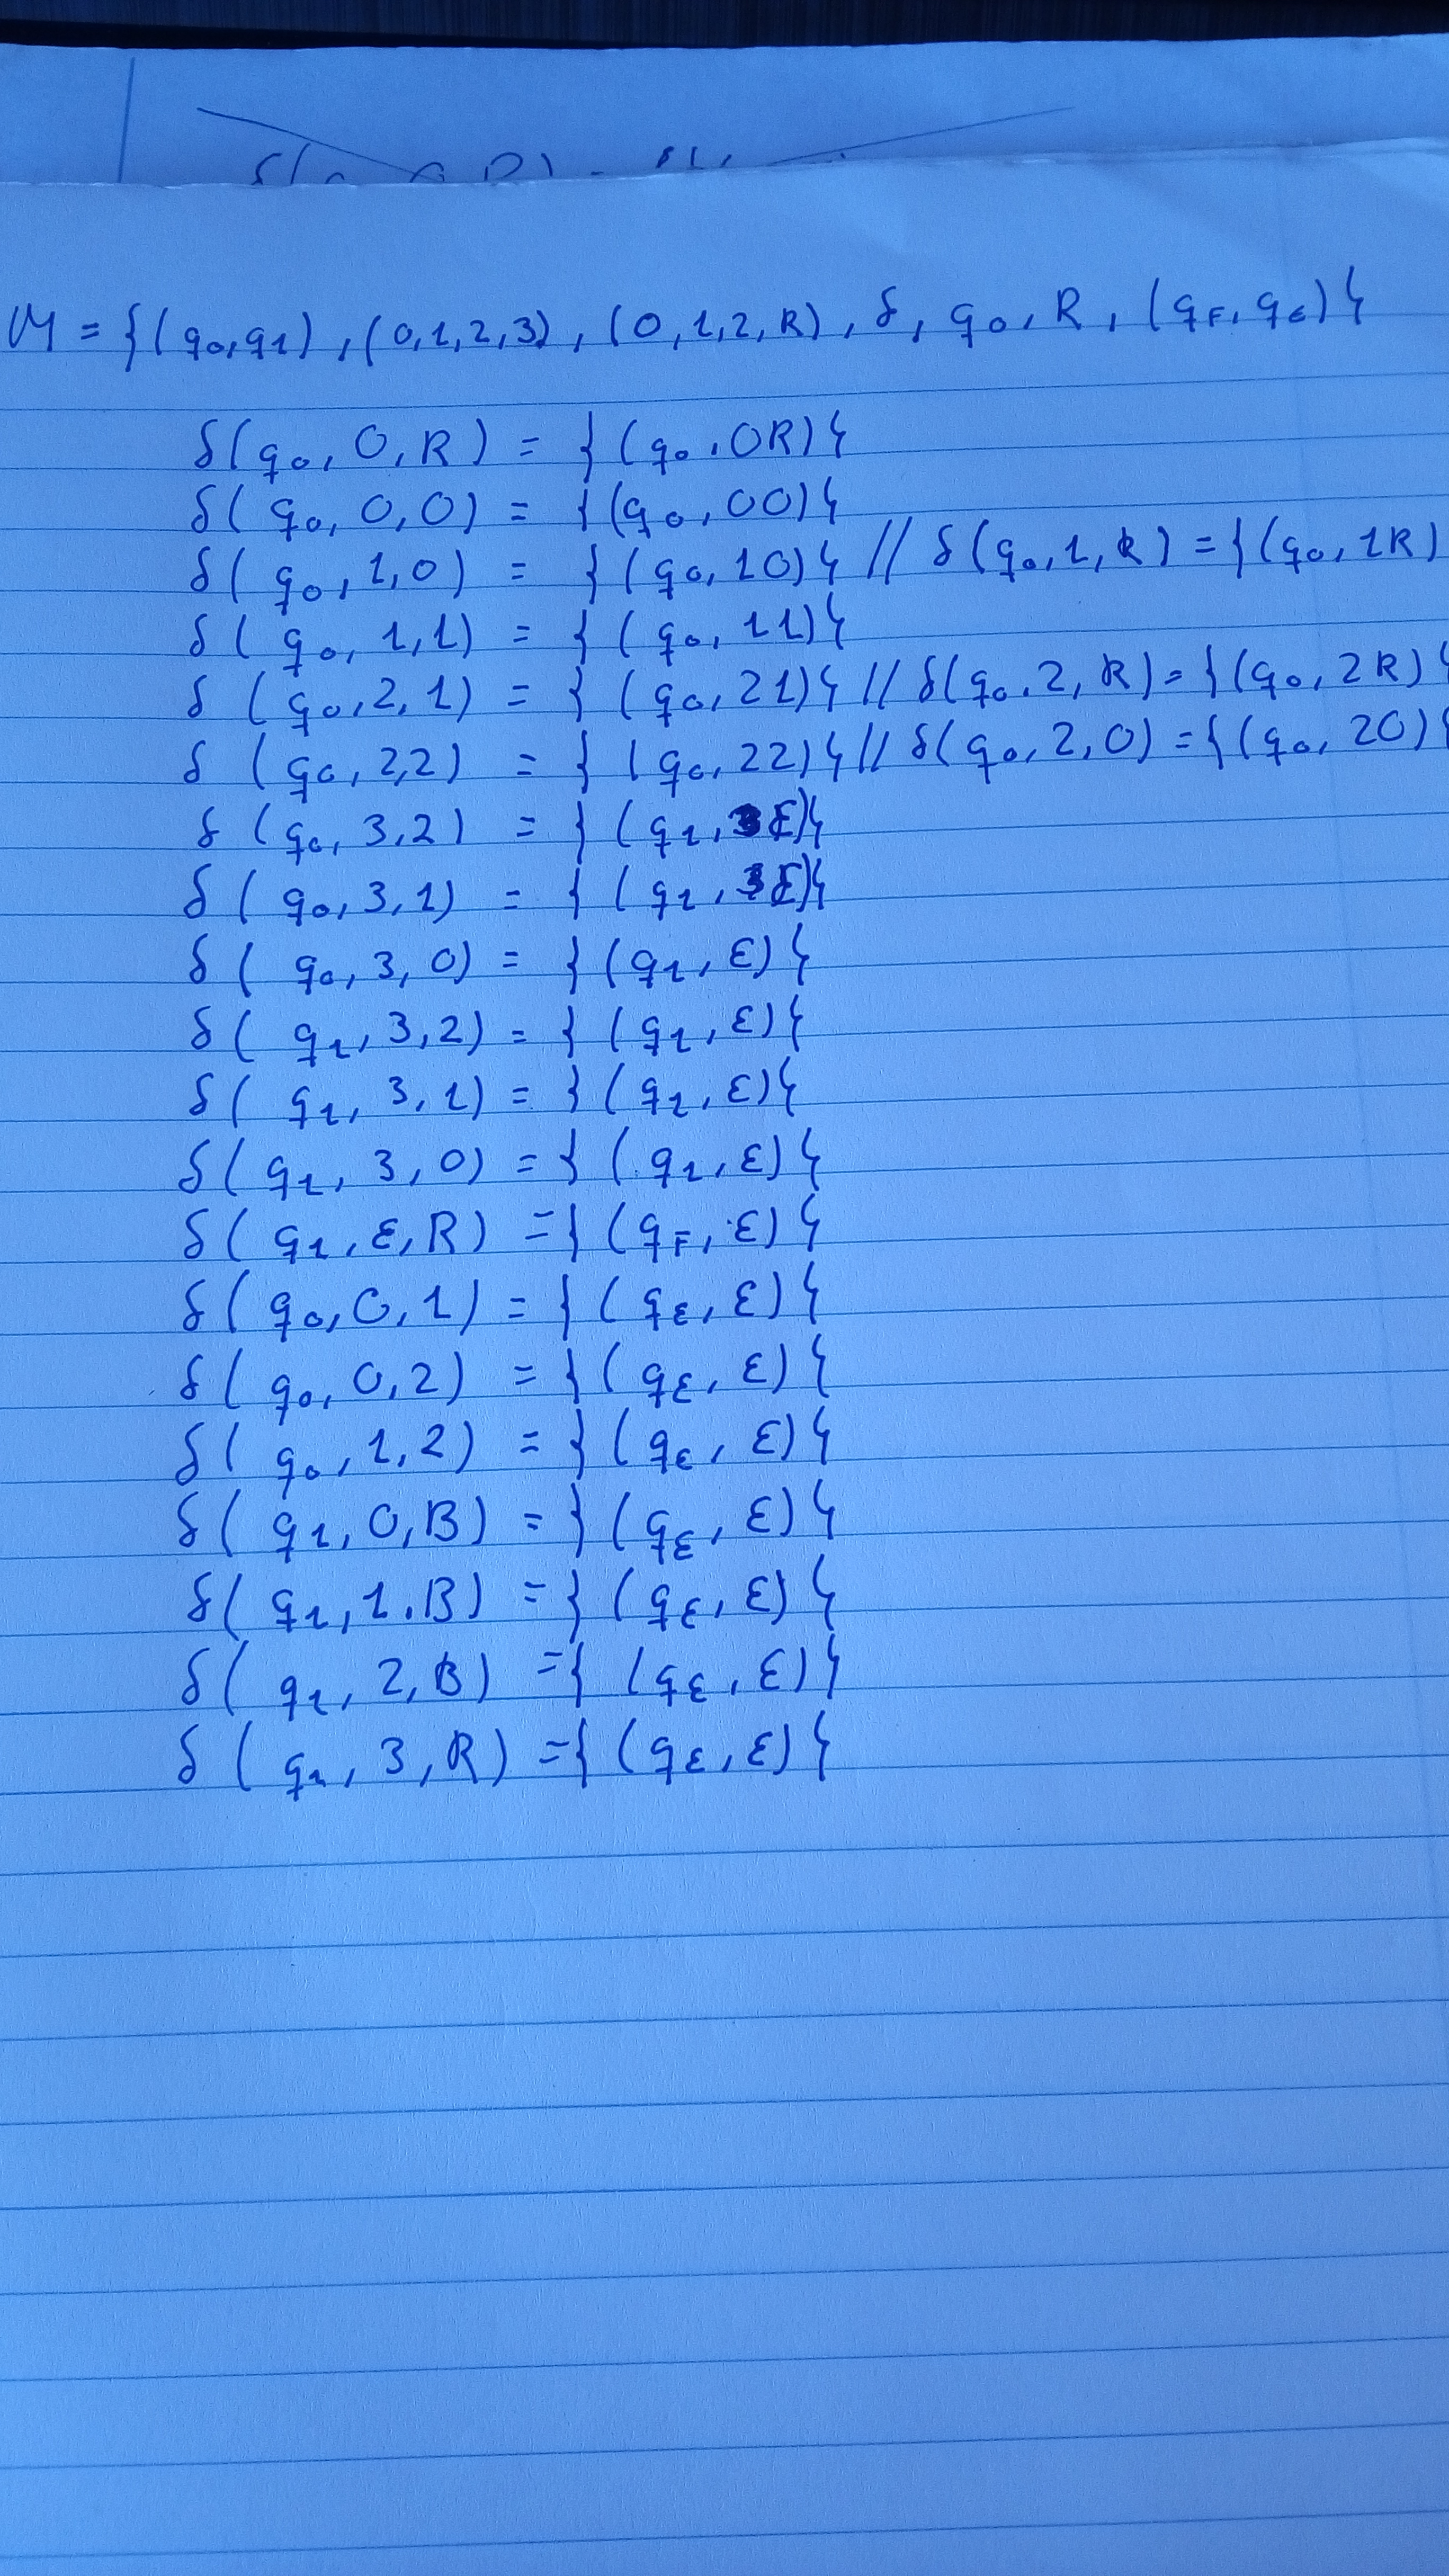
\includegraphics[scale=0.1]{fotos/ej21}
  \end{figure}
  \subsubsection{2}
  \begin{figure}[H]
    \centering
    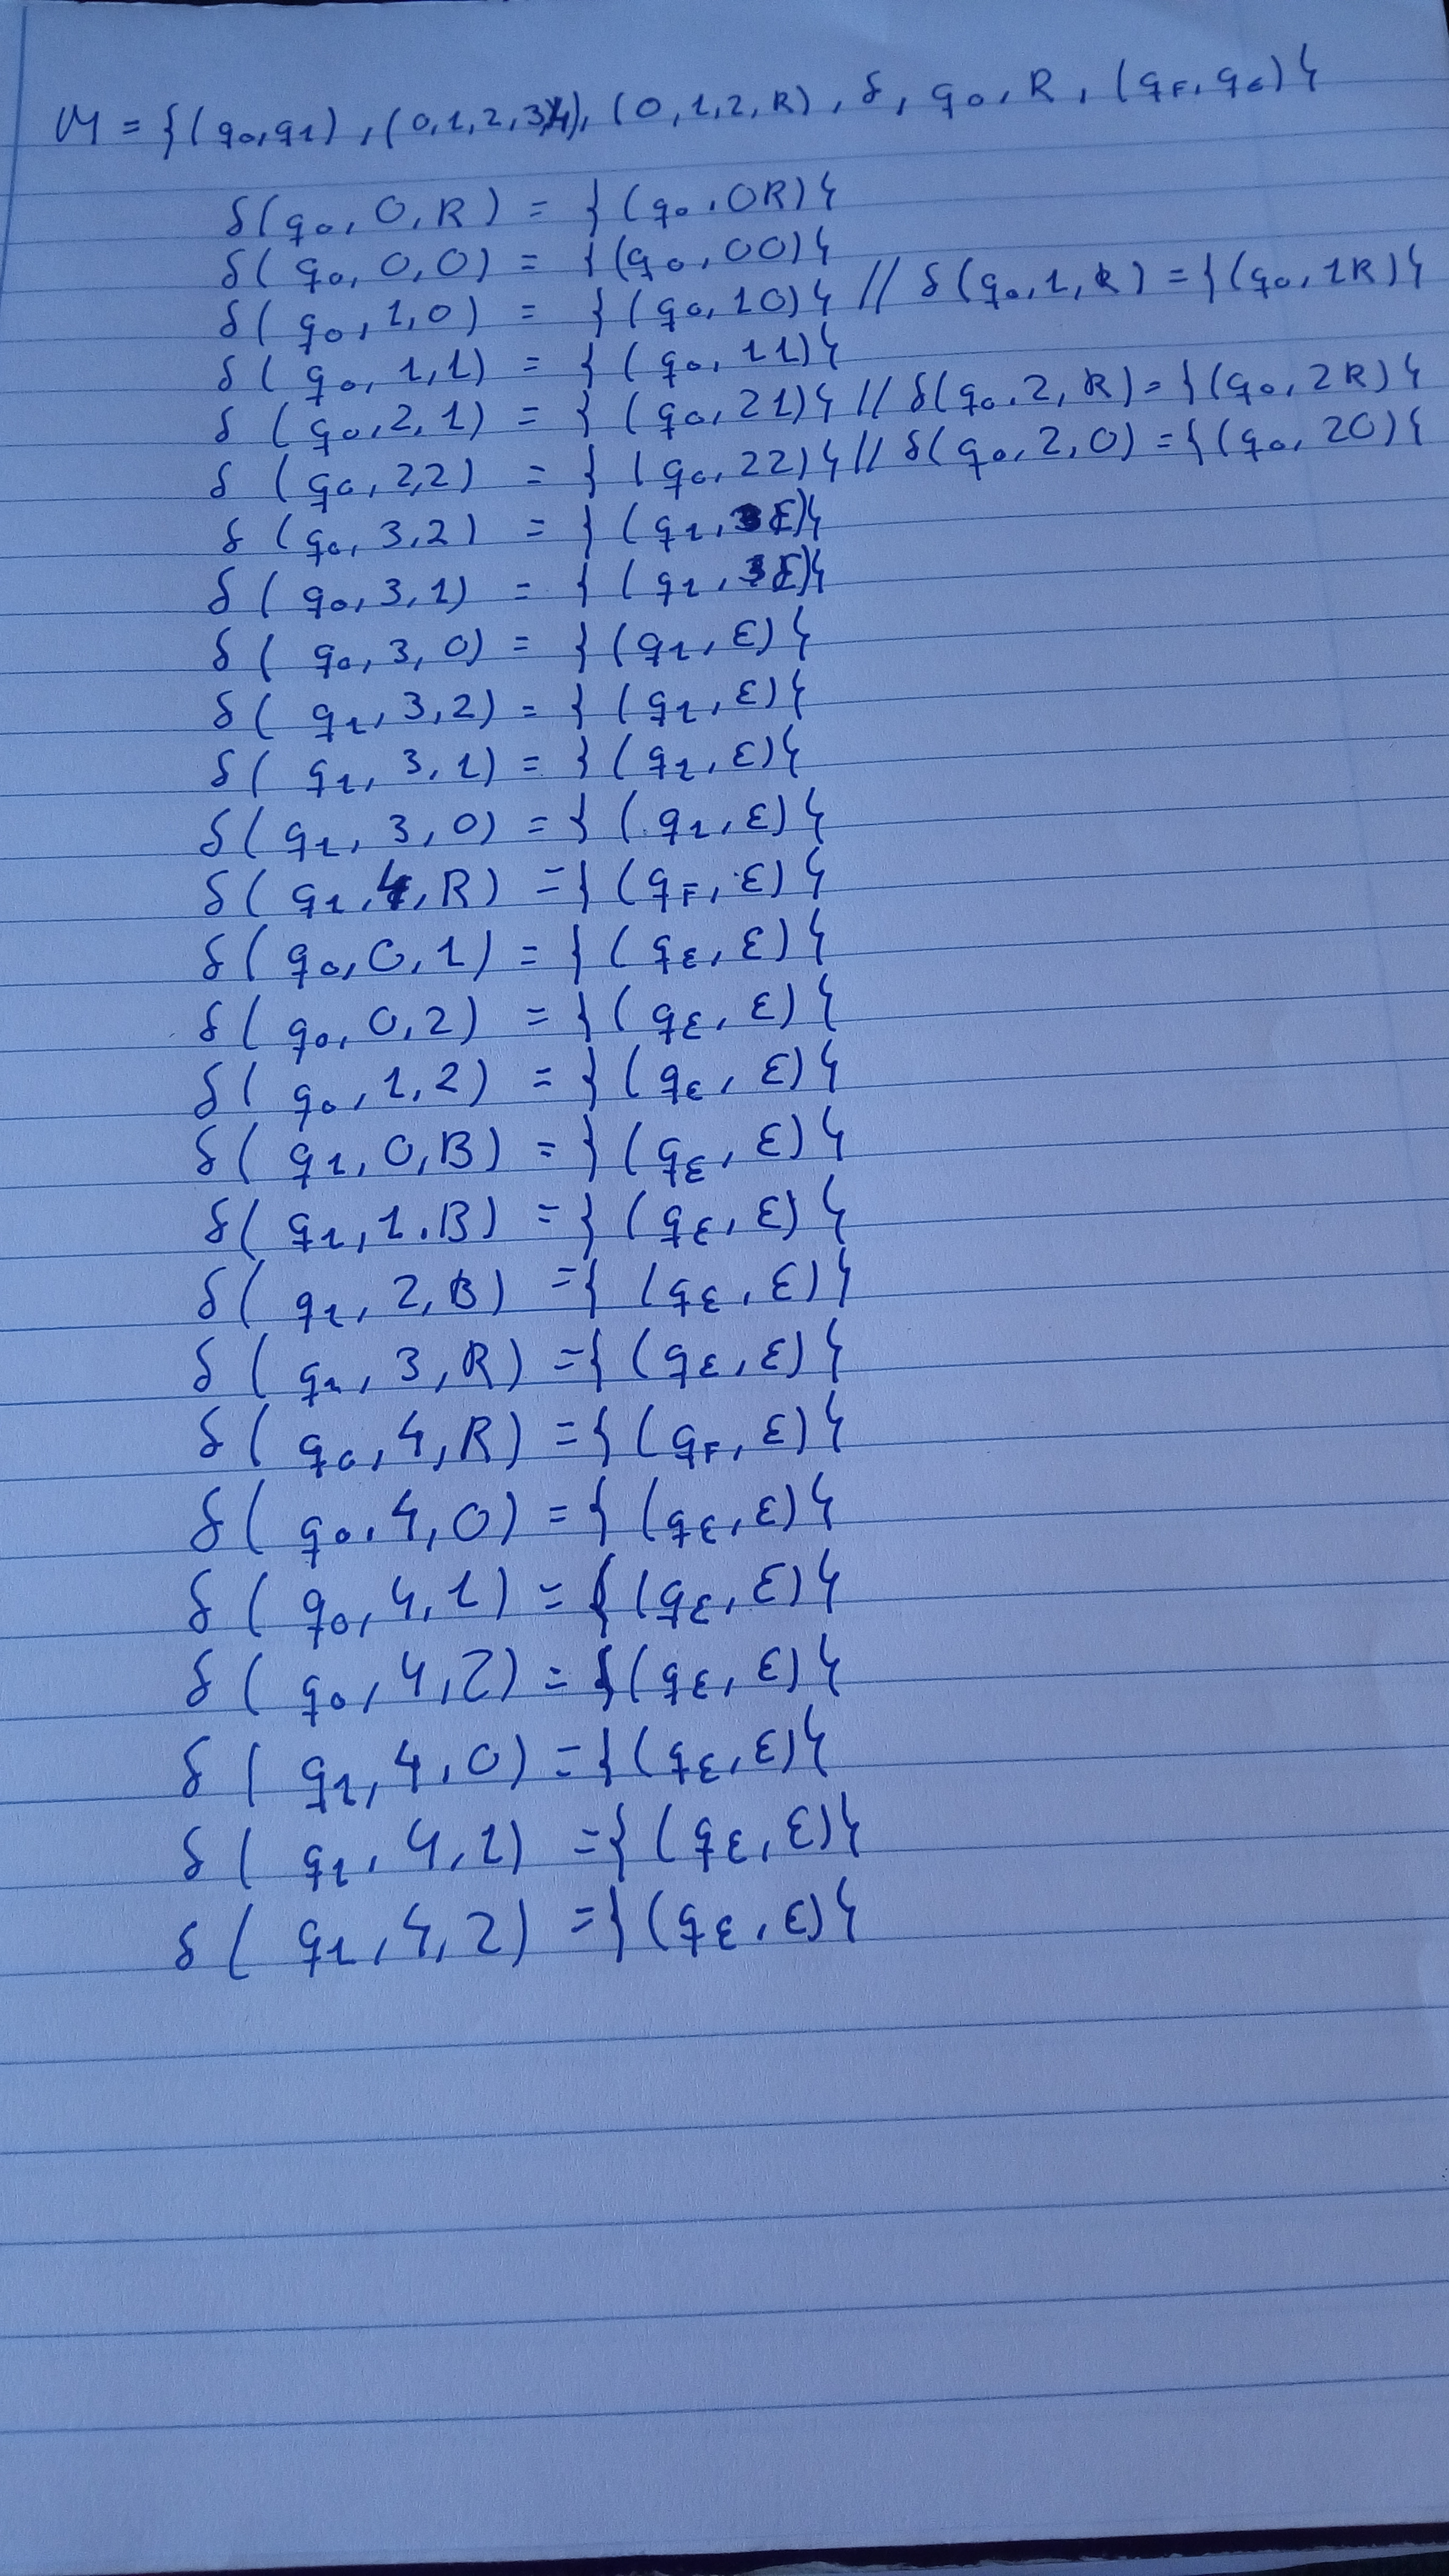
\includegraphics[scale=0.1]{fotos/ej22}
  \end{figure}

\end{document}
